\documentclass[border=2pt]{standalone}
% Shared TikZ styles for the memory-architecture diagrams (compiled as standalone PDFs).
\usepackage[T1]{fontenc}
\usepackage{lmodern}
\usepackage[english]{babel}
\usepackage{tikz}
\usetikzlibrary{positioning,fit,arrows.meta,calc,backgrounds,shapes.geometric}
\definecolor{procFill}{HTML}{E8F1FB}\definecolor{procLine}{HTML}{2A78D6}
\definecolor{memFill}{HTML}{EAF7F1}\definecolor{memLine}{HTML}{1BAF7A}
\definecolor{wFill}{HTML}{FFF6E0}\definecolor{wLine}{HTML}{EDA100}
\definecolor{slowRed}{HTML}{E34948}\definecolor{boxLine}{HTML}{9A9890}\definecolor{ink2}{HTML}{52514E}
\tikzset{
  every node/.style={font=\small, align=center},
  proc/.style={rectangle, rounded corners=2pt, draw=procLine, fill=procFill, very thick, minimum height=2.4em, inner sep=3pt},
  mem/.style={rectangle, draw=memLine, fill=memFill, very thick, inner sep=4pt},
  weights/.style={rectangle, draw=wLine, fill=wFill, thick, font=\footnotesize, inner sep=2pt},
  box/.style={draw=boxLine, dashed, rounded corners=3pt, inner sep=6pt},
  boxlabel/.style={font=\footnotesize\bfseries, text=ink2},
  bus/.style={line width=#1, ink2},
  buslabel/.style={font=\footnotesize, text=ink2, fill=white, inner sep=1pt},
}

\begin{document}
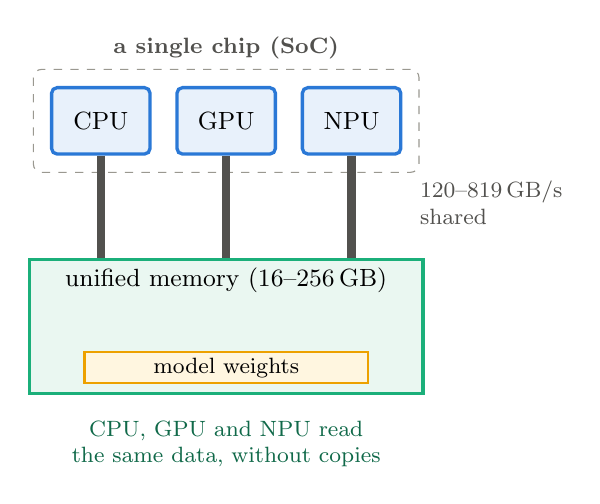
\begin{tikzpicture}
  \node[proc, minimum width=1.25cm] (cpu) {CPU};
  \node[proc, minimum width=1.25cm, right=3mm of cpu] (gpu) {GPU};
  \node[proc, minimum width=1.25cm, right=3mm of gpu] (npu) {NPU};
  \begin{scope}[on background layer]
    \node[box, fit=(cpu)(gpu)(npu), label={[boxlabel]above:a single chip (SoC)}] (soc) {};
  \end{scope}
  \node[mem, minimum width=5.0cm, minimum height=1.7cm, below=13mm of gpu] (mem) {};
  \node[font=\small, anchor=north] at (mem.north) {unified memory (16--256\,GB)};
  \node[weights, minimum width=3.6cm, anchor=south] at ([yshift=4pt]mem.south) {model weights};
  \draw[bus=3pt] (cpu.south) -- (cpu.south |- mem.north);
  \draw[bus=3pt] (gpu.south) -- (gpu.south |- mem.north);
  \node[font=\footnotesize, text=ink2, right=1mm of npu.south east, anchor=north west, yshift=-2mm, align=left] {120--819\,GB/s\\shared};
  \draw[bus=3pt] (npu.south) -- (npu.south |- mem.north);
  \node[font=\footnotesize, text=memLine!60!black, below=2mm of mem] {CPU, GPU and NPU read\\the same data, without copies};
\end{tikzpicture}
\end{document}
